\documentclass[12pt]{article}
\usepackage{amsmath}
\usepackage{tikz}
\usepackage{multicol}
\usepackage{enumitem}
\usepackage{graphicx}
\usepackage{pgfplots}
\pgfplotsset{compat=1.17}

\title{\textbf{Trigonometry}}
\author{Tutoring Centre Ferndale\\\includegraphics[width=4em]{ApS_logo.png}}

\date{}

\begin{document}

\maketitle

Trigonometry is the study of the relationships between the angles and sides of triangles, particularly right-angled triangles. Trigonometry is a Greek word that means "three side measuring." It has wide applications in various fields such as physics, engineering, and astronomy.

\section*{The Unit Circle}
The unit circle is a circle with a radius of 1 centered at the origin of the coordinate plane. It is defined by the equation:
$$x^2 + y^2 = 1$$
where \(x\) and \(y\) are the coordinates of any point on the circle.

\begin{center}
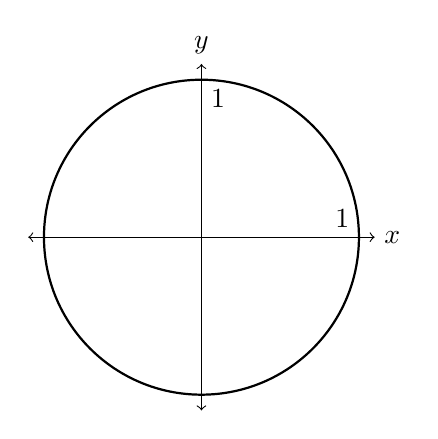
\begin{tikzpicture}
    % Draw the unit circle
    \draw[thick] (0,0) circle(2);
    \draw[<->] (-2.2,0) -- (2.2,0) node[right] {$x$};
    \draw[<->] (0,-2.2) -- (0,2.2) node[above] {$y$};
    \node[above left] at (2,0) {1};
    \node[below right] at (0,2) {1};
\end{tikzpicture}
\end{center}

It is a fundamental tool in trigonometry because it provides a reference for the measurement of angles and other geometric shapes.\\

\section*{Angles}
\begin{itemize}
    \item \textbf{A point} is a specific location in space with no dimensions — no length, width, or height. In the coordinate plane, a point is defined by a pair of coordinates (x,y), which specify its position relative to the origin.
    \item \textbf{A line} is a straight, continuous set of points that extends infinitely in both directions. It is defined by a linear equation in the form y=mx+c, where m is the slope and c is the y-intercept.
    \item A line segment is a part of a line that is bounded by two distinct endpoints. It contains all the points on the line that lie between those two endpoints. A line segment has a finite length.
    \item \textbf{A ray} is a part of a line that starts at an endpoint and extends infinitely in one direction.
    \item \textbf{An angle} is formed by two rays or line segments that share a common endpoint, known as the vertex.

\vfill

    \item  An angle is measured by the amount of rotation from the initial side (starting ray) to the terminal side (ending ray).

\begin{center}
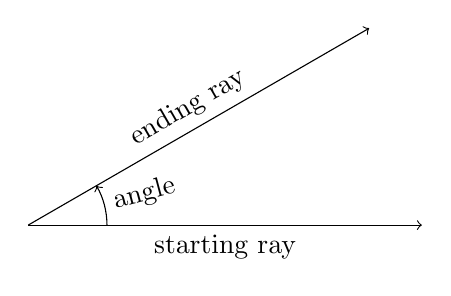
\begin{tikzpicture}
\draw [->] (0,0) -- (5,0)
node[midway,sloped,below]{starting ray};
\draw [->] (0,0) -- ({cos(30)*5},{sin(30)*5})
node[midway,sloped,above]{ending ray};
\draw[->,thin] (1,0) arc (0:30:1)
node[midway,right,rotate=15]{angle};
\end{tikzpicture}
\end{center}
\newpage

    \item Angles can be measured in degrees or radians or gradians.
    \begin{itemize}
        \item \textbf{A degree} is $\frac{1}{360}^{\textrm{th}}$ of a full circle.
        \item \textbf{A radian} is the angle made by extending the length of one radius along the circumference of a circle between the starting and ending rays.
        \item Since $\pi$ is defined as the ratio between the circumference and the diameter of a circle, $\pi=\frac{C}{D}$, and the diameter of a circle is twice the radius, $\pi=\frac{C}{2r}$, there are $2\pi$ radii in a full circle.
        \item $1$ radian $\approx 57.3^{\circ}$.
        \item \textbf{A gradian} (also known as a gon or a grade) is $\frac{1}{400}^{\textrm{th}}$ of a circle. Gradians are less commonly used than degrees and radians, particularly outside of Europe.
    \end{itemize}
\end{itemize}

\begin{center}
\begin{tikzpicture}[scale=4]
    % Draw the unit circle
    \draw[dashed] (0,0) circle(1);
    % Draw the starting ray
    \draw[->, thick] (0,0) -- (1,0) node[midway,sloped,below] {starting ray};
    % Draw the ending ray for 1 radian
    \draw[->, thick] (0,0) -- ({cos(57.3)}, {sin(57.3)}) node[midway,sloped,above] {ending ray};
    % Draw the angle arc
    \draw[thick] (1,0) arc (0:57.3:1) node[midway,sloped,above]{1 radius};
    % Draw the label
    \draw[->] (0.4,0) arc (0:57.3:0.4);
    \node[right] at (30:0.45) {1 radian};
    %Draw 360
    \draw[->] (0.174,0) arc (0:350:0.174) ;
    \node at (200:0.45) {$360$ degrees};
    \node [above] at (0,1.2){$\frac{\pi}{2}$ radians};
    \node [left] at (-1.1,0){$\pi$ radians};
    \node [below] at (0,-1.1){$\frac{3\pi}{2}$ radians};
    \node [anchor=north west] at (1.2,0){$2\pi$ radians};
    % Draw the axes
    \draw[<->] (-1.1,0) -- (1.1,0) node[right] {$x$};
    \draw[<->] (0,-1.1) -- (0,1.1) node[above] {$y$};
\end{tikzpicture}
\end{center}

\newpage

\section*{Angles in Standard Position}

An angle is in standard position when it is drawn in the coordinate plane with its vertex at the origin \((0, 0)\) and its initial side along the positive \(x\)-axis. 

\begin{itemize}
\item \textbf{Initial Side:} The initial side of the angle is always placed along the positive \(x\)-axis.
\item \textbf{Terminal Side:} The terminal side is the ray that rotates about the vertex (the origin) to form the angle. The amount of rotation determines the measure of the angle.

\item \textbf{Sign of the Angle:}
    \begin{itemize}
    \item Counterclockwise Rotation: If the terminal side rotates counterclockwise from the initial side, the angle is considered positive.
    \item Clockwise Rotation: If the terminal side rotates clockwise, the angle is considered negative.
    \end{itemize}

\begin{center}
\begin{minipage}{0.45\textwidth}
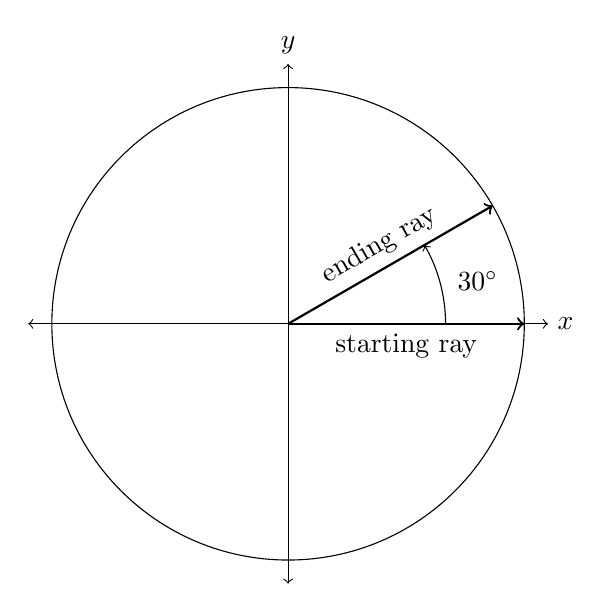
\begin{tikzpicture}
    % Draw the unit circle
    \draw (0,0) circle(3);
    % Draw the starting ray
    \draw[->, thick] (0,0) -- (3,0) node[midway,sloped,below] {starting ray};

    %Draw positive angle
    \draw[->, thick] (0,0) -- ({cos(30)*3}, {sin(30)*3}) node[midway,sloped,above] {ending ray};
    \draw[thin,->] (2,0) arc (0:30:2) ;
    \node[right] at (15:2.1) {$30^{\circ}$};

    % Draw the axes
    \draw[<->] (-3.3,0) -- (3.3,0) node[right] {$x$};
    \draw[<->] (0,-3.3) -- (0,3.3) node[above] {$y$};
\end{tikzpicture}
\end{minipage}
\hfill
\begin{minipage}{0.45\textwidth}
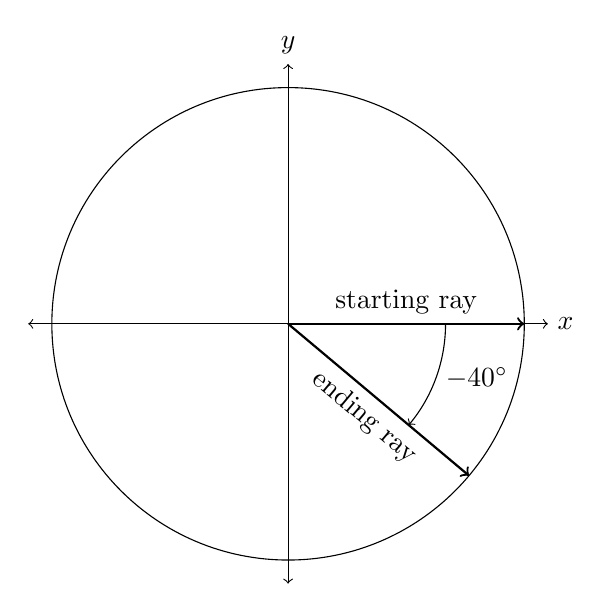
\begin{tikzpicture}
    % Draw the unit circle
    \draw (0,0) circle(3);

    % Draw the starting ray
    \draw[->, thick] (0,0) -- (3,0) node[midway,sloped,above] {starting ray};

    %Draw negative angle
    \draw[->, thick] (0,0) -- ({cos(320)*3}, {sin(320)*3}) node[midway,sloped,below] {ending ray};
    \draw[thin,->] (2,0) arc (0:-40:2);
    \node[right] at (340:2) {$-40^{\circ}$};

    % Draw the axes
    \draw[<->] (-3.3,0) -- (3.3,0) node[right] {$x$};
    \draw[<->] (0,-3.3) -- (0,3.3) node[above] {$y$};
\end{tikzpicture}
\end{minipage}
\end{center}

\item \textbf{The Greek letter theta $\theta$} is commonly used in trigonometry to label angles. It was originally chosen, perhaps, because it is composed of a circle and a line which suggests the idea of an angle or part of a circle.
\item \textbf{Degrees} are abbreviated as a small raised circle, originally chosen, perhaps, because a degree is a measure of a circle.

\item  \textbf{Quadrants:} Depending on the rotation, the terminal side of the angle may lie in one of the four quadrants of the coordinate plane:
    \begin{itemize}
    \item First Quadrant: If the terminal side is between the positive \(x\)-axis and the positive \(y\)-axis.
    \item Second Quadrant: If the terminal side is between the positive \(y\)-axis and the negative \(x\)-axis.
    \item Third Quadrant: If the terminal side is between the negative \(x\)-axis and the negative \(y\)-axis.
    \item Fourth Quadrant: If the terminal side is between the negative \(y\)-axis and the positive \(x\)-axis.
\end{itemize}
\end{itemize}

\begin{center}
\begin{tikzpicture}
    % Draw unit circle
    \draw (0,0) circle(5);
    % Draw axes
    \draw[<->] (-5.5,0) -- (5.5,0) node[right] {$+x$};
    \draw[<->] (0,-5.5) -- (0,5.5) node[above] {$+y$};
    \draw[<->] (5.5,0) -- (-5.5,0) node[left] {$-x$};
    \draw[<->] (0,5.5) -- (0,-5.5) node[below] {$-y$};    % Label quadrants
    \node[align=center] at (45:3) {First Quadrant \\ (+,+)};
    \node[align=center] at (135:3) {Second Quadrant \\ (-,+)};
    \node[align=center] at (225:3) {Third Quadrant \\ (-,-)};
    \node[align=center] at (315:3) {Fourth Quadrant \\ (+,-)};
\end{tikzpicture}
\end{center}

\newpage

\section*{Sine and Cosine}
For any angle \(\theta\) measured from the positive x-axis, the coordinates of the corresponding point on the unit circle are the sine and cosine of $\theta$, abbreviated \((\cos \theta, \sin \theta)\).\\

Sine is a Latin word for curve that is a mistranslation of an Arabic word for bowstring.\\

\begin{center}
\begin{tikzpicture}[scale=3.5]
    % Draw the unit circle
    \draw[thin] (0,0) circle(1);
    % Draw the angle
    \draw[->, thick] (0,0) -- (1,0)
    node[anchor=north west] {1};
    \draw[->, thick] (0,0) -- ({cos(30)}, {sin(30)}) node[anchor=south west] {$(\cos \theta, \sin \theta)$};
    % Draw the angle arc
    \draw[->,thin] (0.2,0) arc (0:30:0.2);
    \node at (15:0.3) {$\theta$};
    \draw[dashed](0,{sin(30)}) -- ({cos(30)},{sin(30})
    node[midway,sloped,above]{cosine};
    \draw[dashed]({cos(30)},0) -- ({cos(30)},{sin(30)})
    node[midway,sloped,above]{sine};
    % Label the axes
    \draw[<->] (-1.2,0) -- (1.2,0) node[right] {$x$};
    \draw[<->] (0,-1.2) -- (0,1.2) node[above] {$y$};
\end{tikzpicture}
\end{center}

\subsection*{Inverse Functions}
\begin{itemize}
    \item The \textbf{arcsine} (arcsin) or \textbf{$\sin^{-1}$} is the inverse of the sine, giving the angle whose sine is a given value.
    \item The \textbf{arccosine} (arccos) or \textbf{$\cos^{-1}$} is the inverse of the cosine, giving the angle whose cosine is a given value.
    \item The \textit{arc-} prefix refers to the arc of the unit circle measured between the rays of an angle.
\end{itemize}

\newpage

\section*{The Sine Function}
The sine function is defined as:
\[
y = \sin(x)
\]
The graph of the sine function is a smooth, periodic curve that oscillates between $y = -1$ and $y = 1$. The period of the sine function is $2\pi$, meaning that the function repeats itself every $2\pi$ units along the x-axis.

\begin{center}
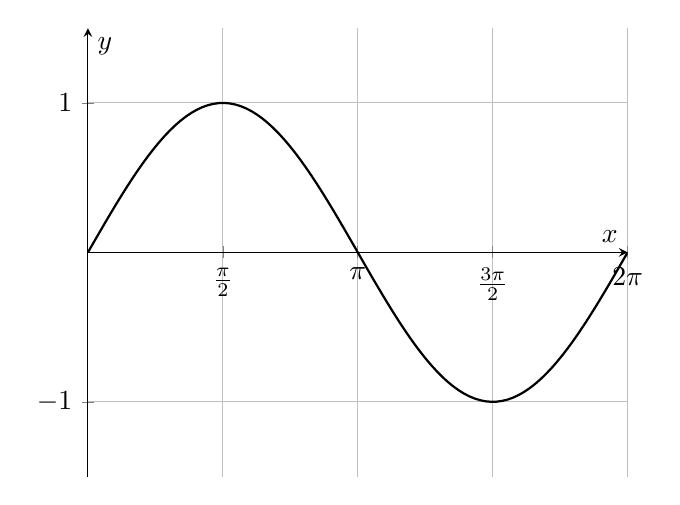
\begin{tikzpicture}
\begin{axis}[
    axis lines = middle,
    xlabel = {$x$},
    ylabel = {$y$},
    ymin = -1.5, ymax = 1.5,
    samples=100,
    domain=0:2*pi,
    xtick={0, pi/2, pi, 3*pi/2, 2*pi},
    xticklabels={$0$, $\frac{\pi}{2}$, $\pi$, $\frac{3\pi}{2}$, $2\pi$},
    ytick={-1,1},
    grid=both,
]
\addplot [thick] {sin(deg(x))};
\end{axis}
\end{tikzpicture}
\end{center}

The general form of the sine function is:
\[
y = A \sin(Bx + C) + D
\]
where:
\begin{itemize}
    \item $A$ is the amplitude (the maximum height of the wave).
    \item $B$ affects the period (the wave frequency, which is $\frac{2\pi}{|B|}$).
    \item $C$ causes a horizontal shift.
    \item $D$ causes a vertical shift.
\end{itemize}

\newpage

\section*{The Cosine Function}
The cosine function is defined as:
\[
y = \cos(x)
\]
Like the sine function, the cosine function oscillates between $y = -1$ and $y = 1$ with a period of $2\pi$.

\begin{center}
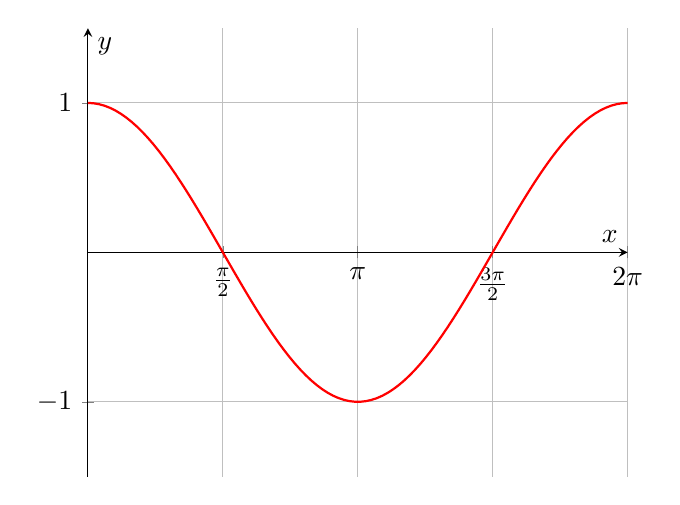
\begin{tikzpicture}
\begin{axis}[
    axis lines = middle,
    xlabel = {$x$},
    ylabel = {$y$},
    ymin = -1.5, ymax = 1.5,
    samples=100,
    domain=0:2*pi,
    xtick={0, pi/2, pi, 3*pi/2, 2*pi},
    xticklabels={$0$, $\frac{\pi}{2}$, $\pi$, $\frac{3\pi}{2}$, $2\pi$},
    ytick={-1,1},
    grid=both,
]
\addplot [red, thick] {cos(deg(x))};
\end{axis}
\end{tikzpicture}
\end{center}

The general form of the cosine function is similar to the sine function:
\[
y = A \cos(Bx + C) + D
\]
The parameters $A$, $B$, $C$, and $D$ have the same effects on the cosine function as they do on the sine function.

\newpage

\section*{Tangent and Cotangent}
\begin{itemize}
\item The tangent of the angle \(\theta\) is the ratio of the sine to the cosine:
\[ \tan \theta = \frac{\sin \theta}{\cos \theta}\]

\item The cotangent of the angle \(\theta\) is the ratio of the cosine to the sine:

\[\cot \theta = \frac{\cos \theta}{\sin \theta}\]
\end{itemize}

Given the equation of a line $y=mx+b$ where $m$ is the slope $m=\frac{rise}{run}$, the tangent can be interpreted as the slope of the line connecting the origin to the point \((\cos \theta, \sin \theta)\) on the unit circle.

\begin{center}
\begin{tikzpicture}[scale=4]
    % Draw the unit circle
    \draw[thin] (0,0) circle(1);
    % Draw the angle
    \draw[->, thick] (0,0) -- (1,0)
    node[anchor=north west] {1};
    % Terminal side for the angle
    \draw[->, thick] (0,0) -- ({cos(30)},{sin(30)})
    node[midway,above,sloped]{$y=\frac{sin\theta}{cos\theta}=tan\theta$};
    % Draw the angle arc
    \draw[thin,->] (0.2,0) arc (0:30:0.2);
    \node at (15:0.3) {$\theta$};
    % Label the axes
    \draw[<->] (-1.2,0) -- (1.2,0) node[right] {$x$};
    \draw[<->] (0,-1.2) -- (0,1.2) node[above] {$y$};
\end{tikzpicture}
\end{center}

\newpage

\begin{itemize}
\item Tangent is from a Latin word that means to touch. A tangent is any line that touches a circle at a single point without crossing it.
\item In trigonometry, the tangent and cotangent of an angle can be visualized in two ways:
\begin{itemize}
    \item The tangent of an angle is the length of a vertical line tangent to the unit circle from the x-axis to the terminating ray.\\
    The cotangent of an angle is the length of a horizontal line tangent to the unit circle from the y-axis to the terminating ray.\\
    \item The tangent of an angle is the length, from the x-axis to the terminating ray, of a line tangent to the unit circle at the point of intersection of the terminating ray.\\
    The cotangent of an angle is the length, from the y-axis to the terminating ray, of a line tangent to the unit circle at the point of intersection of the terminating ray.
\end{itemize}
\end{itemize}
\begin{minipage}{0.5\textwidth}
\begin{tikzpicture}[scale=2.8]
    % Draw the unit circle
    \draw[thin] (0,0) circle(1);
    % Draw the angle
    \draw[->, thin] (0,0) -- (1,0)
    node[anchor=north west] {1};
    % Terminal side for the angle
    \draw[->, thin] (0,0) -- ({cot(30)},1);
    % Draw the angle arc
    \draw[thin,->] (0.2,0) arc (0:30:0.2);
    \node at (15:0.3) {$\theta$};
    % Draw the tangent line
    \draw[thick] (1,0) -- (1,{tan(30)})
    node[midway,sloped,below]{tangent};
    % Draw the cotangent line
    \draw[thick] (0,1) -- ({cot(30)},1)
    node[midway,above] {cotangent};
    % Label the axes
    \draw[<->] (-1.2,0) -- (1.2,0) node[right] {$x$};
    \draw[<->] (0,-1.2) -- (0,1.2) node[above] {$y$};
\end{tikzpicture}
\end{minipage}
\hfill
\begin{minipage}{0.5\textwidth}
\begin{tikzpicture}[scale=2.5]
    % Draw the unit circle
    \draw[thin] (0,0) circle(1);
    % Draw the angle
    \draw[->, thin] (0,0) -- (1,0)
    node[anchor=north west] {1};
    % Terminal side for the angle
    \draw[->, thin] (0,0) -- ({cos(30)},{sin(30)});
    % Draw the angle arc
    \draw[thin,->] (0.2,0) arc (0:30:0.2);
    \node at (15:0.3) {$\theta$};
    
    %Draw the tangent line (0,csc(30)) -- (sec(30),0)
    \draw[thick] (0,2) -- (1.1547,0)
    node[pos=0.3,sloped,above]{cotangent}
    node[pos=0.9,sloped,above]{tangent};
    
    % Label the axes
    \draw[<->] (-1.2,0) -- (1.4,0) node[right] {$x$};
    \draw[<->] (0,-1.2) -- (0,2.2) node[above] {$y$};
\end{tikzpicture}
\end{minipage}

\newpage

\subsection*{Inverse Functions}
\begin{itemize}
    \item The \textbf{arctangent} (arctan) or \textbf{$\tan^{-1}$} is the inverse of the tangent, giving the angle whose tangent is a given value.
    \item The \textbf{arccotangent} (arccot) or \textbf{$\cot^{-1}$} is the inverse of the cosine, giving the angle whose cotangent is a given value.
\end{itemize}

\section*{The Tangent Function}
The tangent function is defined as:
\[
y = \tan(x)
\]
Unlike sine and cosine, the tangent function is not bounded. It has vertical asymptotes at $x = \frac{\pi}{2} + n\pi$, where $n$ is an integer. The period of the tangent function is $\pi$, and it repeats every $\pi$ units.

Below is the graph of the tangent function:

\begin{center}
\begin{tikzpicture}
\begin{axis}[
    axis lines = middle,
    xlabel = {$x$},
    ylabel = {$y$},
    ymin = -5, ymax = 5,
    samples=100,
    domain=-pi/2:pi/2,
    xtick={-pi/2, 0, pi/2},
    xticklabels={$-\frac{\pi}{2}$, $0$, $\frac{\pi}{2}$},
    ytick={-4,-2,2,4},
    grid=both,
]
\addplot [thick] {tan(deg(x))};
\end{axis}
\end{tikzpicture}
\end{center}

The general form of the tangent function is:
\[
y = A \tan(Bx + C) + D
\]
The parameters $A$, $B$, $C$, and $D$ influence the tangent function similarly to how they influence the sine and cosine functions, with $B$ affecting the period, $C$ shifting the graph horizontally, and $D$ shifting it vertically. However, the concept of amplitude does not apply to the tangent function as it is unbounded.

\section*{Secant and Cosecant}
\begin{itemize}
\item The secant is the reciprocal of the cosine: $\sec\theta=\frac{1}{\cos\theta}$.

The secant of an angle is the length from the origin to the point on the terminating ray that intersects a vertical line at $x=1$.\\

Secant is a Latin word that means to cut because the secant cuts through the circle.

\item The cosecant is the reciprocal of the sine: $\csc\theta=\frac{1}{\sin\theta}$.

The cosecant of an angle is the length from the origin to the point on the terminating ray that intersects a horizontal line at $y=1$.\\
\end{itemize}

\begin{minipage}{0.45\textwidth}
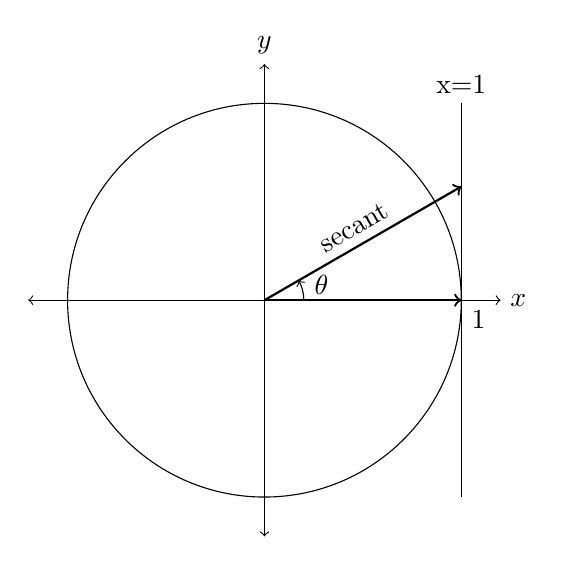
\begin{tikzpicture}[scale=2.5]
    % Draw the unit circle
    \draw[thin] (0,0) circle(1);
    % Draw the angle
    \draw[->, thick] (0,0) -- (1,0)
    node[anchor=north west] {1};
    % Draw the angle arc
    \draw[thin,->] (0.2,0) arc (0:30:0.2);
    \node at (15:0.3) {$\theta$};
    % Draw the tangent line
    \draw[thin] (1,-1) -- (1,1)
    node[above] {x=1};
    % Draw the secant line
    \draw[thick,->] (0,0) -- (1,{tan(30)})
    node[sloped,midway,above] {secant};
    % Label the axes
    \draw[<->] (-1.2,0) -- (1.2,0) node[right] {$x$};
    \draw[<->] (0,-1.2) -- (0,1.2) node[above] {$y$};
\end{tikzpicture}
\end{minipage}
\hfill
\begin{minipage}{0.45\textwidth}
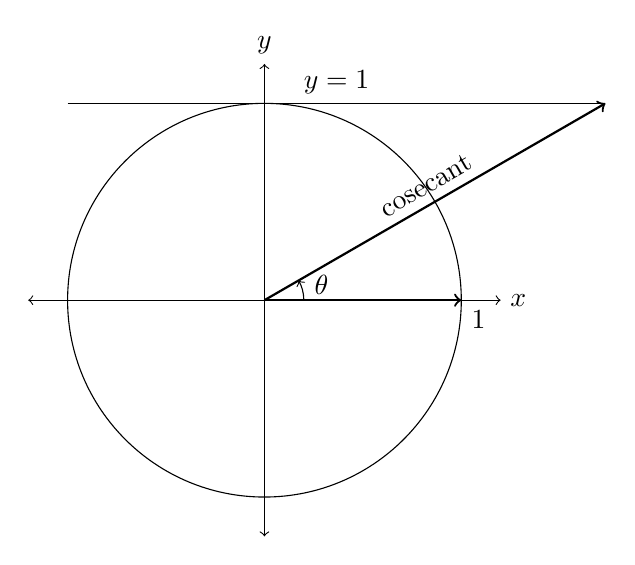
\begin{tikzpicture}[scale=2.5]
    % Draw the unit circle
    \draw[thin] (0,0) circle(1);
    % Draw the angle
    \draw[->, thick] (0,0) -- (1,0)
    node[anchor=north west] {1};
    % Draw the angle arc
    \draw[thin,->] (0.2,0) arc (0:30:0.2);
    \node at (15:0.3) {$\theta$};
    % Draw the tangent line
    \draw[thin] (-1,1) -- ({cot(30)},1)
    node[midway,above]{$y=1$};
    % Draw the cosecant line
    \draw[thick,->] (0,0) -- ({cot(30)},1)
    node[sloped,midway,above] {cosecant};
    % Label the axes
    \draw[<->] (-1.2,0) -- (1.2,0) node[right] {$x$};
    \draw[<->] (0,-1.2) -- (0,1.2) node[above] {$y$};
\end{tikzpicture}
\end{minipage}

\subsection*{Inverse Functions}
\begin{itemize}
    \item The \textbf{arcsecant} (arcsec) or \textbf{$\sec^{-1}$} is the inverse of the secant, giving the angle whose secant is a given value.
    \item The \textbf{arccosecant} (arccsc) or \textbf{$\csc^{-1}$} is the inverse of the cosine, giving the angle whose cotangent is a given value.
\end{itemize}

\section*{SOHCAHTOA}
The sides of a right triangle are named relative to the angle $\theta$ in standard position:

\begin{tikzpicture}[scale=5]
    % Draw the axes
    \draw[<->] (-1.2,0) -- (1.2,0) node[right] {$x$};
    \draw[<->] (0,-1.2) -- (0,1.2) node[above] {$y$};
    % Draw the unit circle
    \draw[thin] (0,0) circle(1);
    % Draw the triangle
    \draw[thick] (0,0) -- ({cos(40)}, {sin(40)}) node[midway, sloped, above]{hypotenuse};
    \draw[thick] ({cos(40)}, {sin(40)}) -- ({cos(40)}, 0) node[midway,xshift=2ex,rotate=270]{opposite};
    \draw[thick] ({cos(40)}, 0) -- (0,0) node[midway, sloped, below]{adjacent};
    % Draw the angle arc
    \draw[thin,->] (0.2,0) arc (0:40:0.2);
    \node at (20:0.3) {$\theta$};
    % Label the right angle
    \draw[thin] ({cos(40)-0.05}, 0) -- ({cos(40)-0.05}, 0.05) -- ({cos(40)}, 0.05);
\end{tikzpicture}

\newpage

\textbf{SOHCAHTOA} stands for:
\begin{center}
\textbf{SOH:} Sine $= \frac{\textrm{Opposite}}{\textrm{Hypotenuse}}$\\
\vspace{8pt}
\textbf{CAH:} Cosine $= \frac{\textrm{Adjacent}}{\textrm{Hypotenuse}}$\\
\vspace{8pt}
\textbf{TOA:} Tangent $= \frac{\textrm{Opposite}}{\textrm{Adjacent}}$\\
\end{center}

\subsection*{Using SOHCAHTOA}
Given a right triangle where:

\begin{itemize}
\item The length of the opposite side is 3
\item The adjacent side is 4
\item The hypotenuse is 5
\end{itemize}

We can calculate the sine, cosine, and tangent of the angle \(\theta\):\\
\begin{center}
\begin{tikzpicture}
    \draw(0,0)--(4,3)node[midway,above]{5};
    \draw(4,3)--(4,0)node[midway,right]{3};
    \draw(4,0)--(0,0)node[midway,below]{4};
    \draw[thin](3.7,0)--(3.7,0.3)--(4,0.3);
    \draw[thin](1,0)arc(0:36.87:1);
    \node at (1.2,0.4){$\theta$};
    \node [anchor=west] at (5,1.5)
    {$\sin \theta = \frac{3}{5},
    \quad \cos \theta = \frac{4}{5},
    \quad \tan \theta = \frac{3}{4};$};
\end{tikzpicture}
\end{center}

The unknown angles can be found using inverse functions:

$$\sin \theta = \frac{3}{5}$$
$$\sin^{-1} \frac{3}{5} \implies \theta \approx36.9^\circ$$

Then, use the fact that angles of a triangle add up to $180^\circ$, so $180-(90+36.9)=53.1^\circ$, or apply SOHCAHTOA to the other angle:

$$\cos (\text{other angle}) = \frac{3}{5}$$
$$\cos^{-1}\frac{3}{5}\implies\text{other angle}\approx53.1^\circ$$

\newpage

\subsection*{Area of a Triangle}
The area of a triangle is half the length of its base times its perpendicular height.\\

Consider a triangle \(ABC\) with sides \(a\), \(b\), and \(c\) opposite vertices \(A\), \(B\), and \(C\), draw a line $h$ perpendicular to the base $c$ of the triangle at $H$ to the vertex of angle $C$. This creates two right triangles. The area of these triangles is given by:
$$Area = \frac{1}{2} \times c \times h.$$

In the right triangle \(HBC\) we have:
$$\sin B = \frac{h}{a} \implies h = a \sin B.$$

Substituting this into the area formula, we get:
$$Area = \frac{1}{2} \times c \times h = \frac{1}{2} \times c \times a \sin B.$$

Thus, the area of the triangle can be expressed as:
$$Area = \frac{1}{2}ac \sin B.$$

\begin{minipage}{0.45\textwidth}
\centering
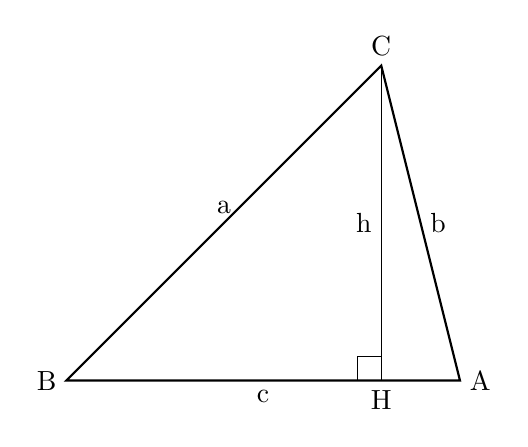
\begin{tikzpicture}
\draw[thick] (0,0) -- (5,0) -- (4,4) -- cycle;
\draw (4,0) -- (4,4) node[midway,left]{h};
\draw[thin] (3.7,0) -- (3.7,0.3) -- (4, 0.3);
\node[below] at (4,0) {H};
\node[right] at (5,0) {A};
\node[left]  at (0,0) {B};
\node[above] at (4,4) {C};
\node[above] at (2,2)   {a};
\node[right] at (4.5,2) {b};
\node[below] at (2.5,0) {c};
\end{tikzpicture}
\end{minipage}%
\hfill
\begin{minipage}{0.45\textwidth}
\centering
\begin{align*}
\text{Area} &= \frac{1}{2}ac \sin B\\
            &= \frac{1}{2}ab \sin C\\
            &= \frac{1}{2}bc \sin A
\end{align*}
\end{minipage}

\newpage

\section*{Special Angles}
\begin{center}
\begin{Large}
\renewcommand{\arraystretch}{1.6}
\begin{tabular}{c|c|c|c}
Angle & sin & cos & tan ($\frac{\text{sin}}{\text{cos}})$\\
\hline
  $0^\circ$ &  0            & 1                    & 0 \\
 $30^\circ$ & $\frac{1}{2}$ & $\frac{\sqrt{3}}{2}$ & $\frac{1}{\sqrt{3}}$ \\
 $45^\circ$ & $\frac{1}{\sqrt{2}}$ & $\frac{1}{\sqrt{2}}$ & $1$ \\
 $60^\circ$ & $\frac{\sqrt{3}}{2}$ & $\frac{1}{2}$ & $\sqrt{3}$ \\
 $90^\circ$ &  1 &  0 & undefined\\
$180^\circ$ &  0 & -1 & 0 \\
$270^\circ$ & -1 &  0 & undefined
\end{tabular}
\end{Large}
\end{center}

\section*{Related Angles}
\begin{center}
\begin{Large}
\renewcommand{\arraystretch}{1.5}
\begin{tabular}{r|c|c}
\hline
$-\theta:$ & $\sin-\theta=-\sin\theta$ & $\cos-\theta= \cos\theta$ \\
\hline
 $90^\circ-\theta:$ & $\sin90^\circ-\theta=\cos\theta$ & $\cos90^\circ-\theta=\sin\theta$ \\
$90^\circ+\theta:$ & $\sin90^\circ+\theta= \cos\theta$ & $\cos90^\circ+\theta=-\sin\theta$ \\
\hline
$180^\circ-\theta:$ & $\sin180^\circ-\theta= \sin\theta$ & $\cos180^\circ-\theta=-\cos\theta$ \\
$180^\circ+\theta:$ & $\sin180^\circ+\theta=-\sin\theta$ & $\cos180^\circ+\theta=-\cos\theta$ \\
\hline
\end{tabular}
\end{Large}
\end{center}

\newpage

\section*{The Sine Rule}
The Sine Rule relates the sides of a triangle to the sines of its angles. It is useful for finding unknown sides or angles in any triangle:

\[\frac{a}{\sin A} = \frac{b}{\sin B} = \frac{c}{\sin C}\]

\subsection*{Using the Sine Rule}

Consider a triangle ABC where:

\begin{itemize}
\item Angle A = 40 degrees
\item Angle B = 60 degrees
\item Side a = 10 units
\end{itemize}

\begin{center}
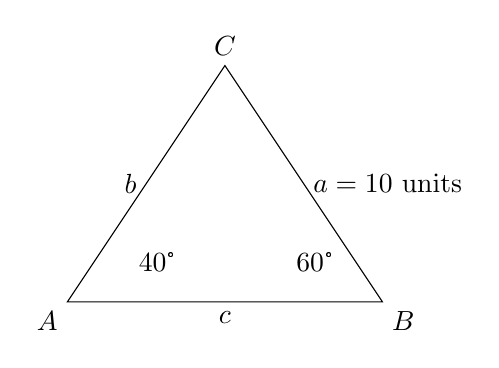
\begin{tikzpicture}
  \draw (0,0) -- (4,0) -- (2,3) -- cycle;
  \draw (0,0) node[below left] {$A$};
  \draw (4,0) node[below right] {$B$};
  \draw (2,3) node[above] {$C$};
  \draw (3,1.5) node[right] {$a=10$ units};
  \draw (1,1.5) node[left] {$b$};
  \draw (2,0) node[below] {$c$};
  \draw (1.5,0.5) node[left] {40°};
  \draw (3.5,0.5) node[left] {60°};
\end{tikzpicture}
\end{center}

We want to find the length of side b.\\

1. Substitute the known values:\\

$$\frac{10}{\sin{40^\circ}} = \frac{b}{\sin{60^\circ}}$$


2. Solve for b:\\

$$b = 10 \cdot \frac{\sin{60^\circ}}{\sin{40^\circ}}
\approx 12.85 \text{ units}$$

\newpage

\section*{The Cosine Rule}
The Cosine Rule relates the sides of a triangle to the cosine of one of its angles. It is useful for finding the length of a side when two sides and the included angle are known:

\[a^2 = b^2 + c^2 - 2bc \cos A\]
\[b^2 = a^2 + c^2 - 2ac \cos B\]
\[c^2 = a^2 + b^2 - 2ab \cos C \]

\vfill

\subsection*{Using The Cosine Rule}

Given a triangle with:
\begin{itemize}
\item Angle C = 60$^\circ$
\item Side a = 5 units
\item Side b = 6 units
\end{itemize}

\begin{center}
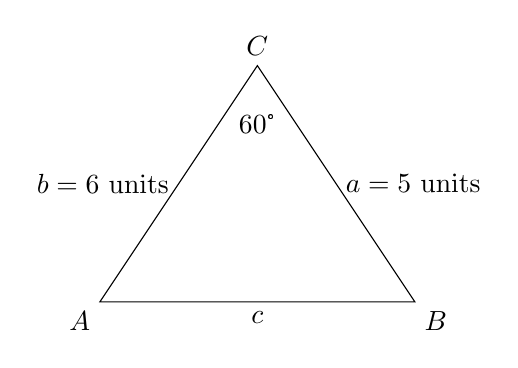
\begin{tikzpicture}
  \draw (0,0) -- (4,0) -- (2,3) -- cycle;
  \draw (0,0) node[below left] {$A$};
  \draw (4,0) node[below right] {$B$};
  \draw (2,3) node[above] {$C$};
  \draw (2,2.5) node[below] {60°};
  \draw (3,1.5) node[right] {$a=5$ units};
  \draw (1,1.5) node[left] {$b=6$ units};
  \draw (2,0) node[below] {$c$};
\end{tikzpicture}
\end{center}

We can find the side \(c\) using the Cosine Rule:

$$c^2 = 5^2 + 6^2 - 2 \times 5 \times 6 \times \cos 60^\circ$$

$$c = \sqrt{25 + 36 - 60 \times \frac{1}{2}} = \sqrt{31} \approx 5.57$$

\newpage

\section*{Trigonometric Identities}
Trigonometric identities are equations involving trigonometric functions that are true for every value of the variable for which both sides are defined. They are  useful for simplifying trigonometric expressions and solving trigonometric equations.

\vfill

\subsection*{The Pythagorean Identity}
The most fundamental trigonometric identity is the Pythagorean identity:
$$\sin^2 \theta + \cos^2 \theta = 1$$
This follows from the Pythagorean Theorem $a^2+b^2=c^2$ and the definition of sine and cosine on the unit circle:
\begin{center}
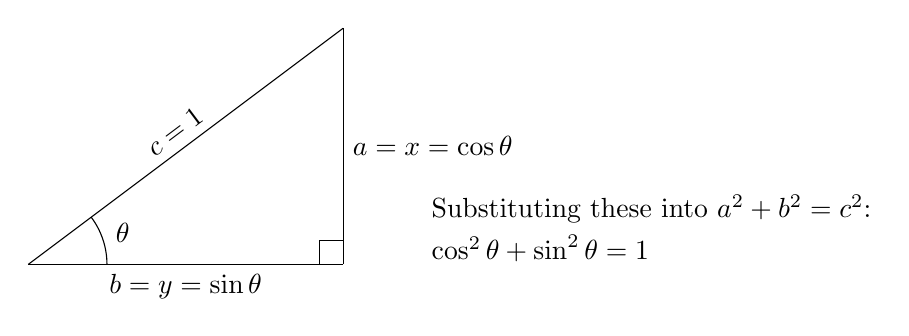
\begin{tikzpicture}
    \draw(0,0)--(4,3)node[sloped,midway,above]{$c=1$};
    \draw(4,3)--(4,0)node[midway,right]{$a=x=\cos \theta$};
    \draw(4,0)--(0,0)node[midway,below]{$b=y=\sin \theta$};
    \draw[thin](3.7,0)--(3.7,0.3)--(4,0.3);
    \draw[thin](1,0)arc(0:36.87:1);
    \node at (1.2,0.4){$\theta$};
    \node [anchor=west] at (5,0.7)
    {Substituting these into $a^2+b^2=c^2$:};
    \node [anchor=west] at (5,0.2)
    {$\cos^2\theta+\sin^2\theta=1$};
\end{tikzpicture}
\end{center}

\vfill

\subsection*{Other Important Identities}
\begin{align*}
1 + \tan^2 \theta &= \sec^2 \theta\\
\sin(2\theta) &= 2 \sin \theta \cos \theta \\
\cos(2\theta) &= \cos^2 \theta - \sin^2 \theta \\
&= 2\cos^2 \theta - 1 \\
&= 1 - 2\sin^2 \theta \\
\tan(2\theta) &= \frac{2 \tan \theta}{1 - \tan^2 \theta}
\end{align*}

\vfill

\newpage

\subsection*{Simplifying Expressions}
For example, consider the expression:
\[
\frac{\sin(2\theta)}{\cos \theta}
\]
We can use the identity for \(\sin(2\theta)\):
\[
\frac{2 \sin \theta \cos \theta}{\cos \theta} = 2 \sin \theta
\]
Thus, the expression simplifies to \(2 \sin \theta\).

\subsection*{Solving Equations}
For example, solve the equation:
\[
\sin^2 \theta - \sin \theta = 0
\]
Factor the equation:
\[
\sin \theta (\sin \theta - 1) = 0
\]
This gives two solutions:
\[
\sin \theta = 0 \quad \text{or} \quad \sin \theta = 1
\]
So, \(\theta = n\pi\) or \(\theta = \frac{\pi}{2} + 2n\pi\) for integer \(n\).

\newpage

\section*{Graphical Solutions}

Graphical solutions are a powerful tool for solving trigonometric equations, especially when algebraic solutions are complex or unknown. By plotting the functions involved and identifying their intersections, we can visually determine approximate solutions.

\subsection*{Example 1: Solving $x + \cos(x) = 0$}

To solve this equation graphically, rewrite it as:
\[
\cos(x) = -x
\]
Then graph the functions $y = \cos(x)$ and $y = -x$ and find their point of intersection.\\

Graph of $y = \cos(x)$ and $y = -x$:

\begin{center}
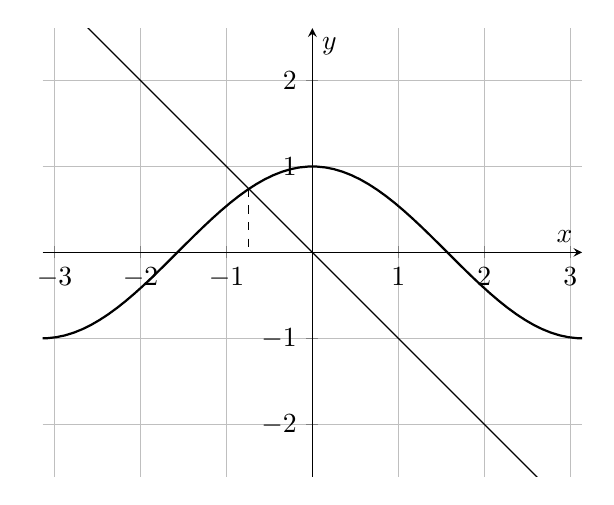
\begin{tikzpicture}
\begin{axis}[
    axis lines = middle,
    xlabel = {$x$},
    ylabel = {$y$},
    ymin = -1.2, ymax = 1.2,
    xmin = -3.14, xmax = 3.14,
    samples=100,
    xtick={-3,-2,-1,0,1,2,3},
    ytick={-2,-1,0,1,2},
    grid=both,
    axis equal
]
\addplot [thick] {cos(deg(x))};
\addplot [thin] {-x};
\draw[dashed](-0.739,0.739) -- (-0.739,0);
\end{axis}
\end{tikzpicture}
\end{center}

The solution to $x + \cos(x) = 0$ is where these two graphs intersect. The intersection occurs near $x \approx 0.74$.

\newpage

\subsection*{Example 2: Solving $\cos(x) = 2x$}

Plot $y = \cos(x)$ and $y = 2x$ and find the intersection.\\

\begin{center}
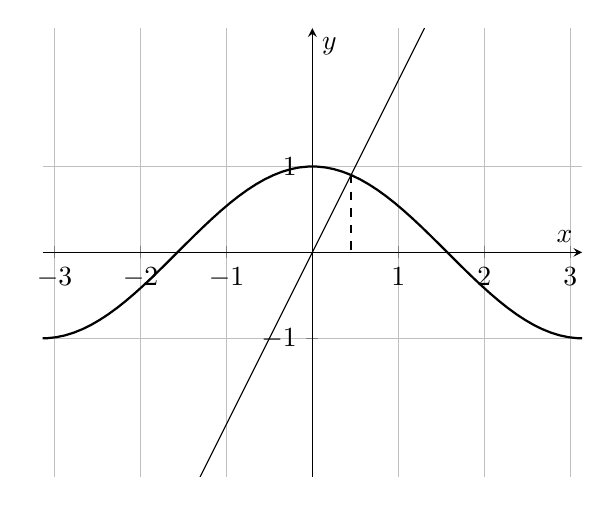
\begin{tikzpicture}
\begin{axis}[
    axis lines = middle,
    xlabel = {$x$},
    ylabel = {$y$},
    ymin = -1.2, ymax = 1.2,
    xmin = -3.14, xmax = 3.14,
    samples=100,
    xtick={-3,-2,-1,0,1,2,3},
    ytick={-1,0,1},
    grid=both,
    axis equal
]
\addplot [thick] {cos(deg(x))};
\addplot [thin] {2*x};
\draw[dashed] (0.45,0.9) -- (0.45,0);
\end{axis}
\end{tikzpicture}
\end{center}

The graphs intersect at $x \approx 0.45$.

\subsection*{Example 3: Solving $\sin(x) = \frac{x}{2}$}

Plot $y = \sin(x)$ and $y = \frac{x}{2}$ to find their intersection:

\begin{center}
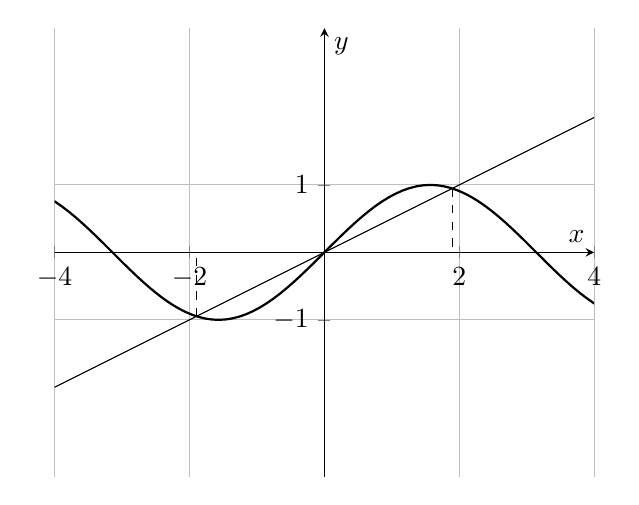
\begin{tikzpicture}
\begin{axis}[
    axis lines = middle,
    xlabel = {$x$},
    ylabel = {$y$},
    ymin = -1.5, ymax = 1.5,
    xmin = -4, xmax = 4,
    samples=100,
    xtick={-4,-2,0,2,4},
    ytick={-1,0,1},
    grid=both,
    axis equal
]
\addplot [thick] {sin(deg(x))};
\addplot [thin] {0.5*x};
\draw[thin,dashed](1.895,0.947) -- (1.895,0);
\draw[thin,dashed](-1.895,-0.947) -- (-1.895,0);
\end{axis}
\end{tikzpicture}
\end{center}

The intersections occur near $x \approx 0.93, x=0,$ and $x\approx0.93.$

\end{document}
